\chapter{Marktsegmente}
Im Kapitel Marktsegmente werden die aktuellen Bereiche von Internet of Things, Smartwatches und Smartwatches im Internet of Things aufgezeigt. Es werden Themen aufgelistet und Bereich davon aufgezeigt. Hierfür ist keine strategische Marktsegmentierung durchgeführt worden, dadurch ist es keine abschliessende Auflistung. Für die Evaluation der Marktsegmente wurde der Bericht, The Internet of Things:
Mapping the value beyond the hype von McKinsey Global Institute als Referenz verwendet (vgl. \cite{mk:iot}).

\section{Marktsegmente im Internet of Things}
\begin{tabbing}
xxxxxxxxxxxxxxxxxxxx\=xxxxxxxxxxxxxxxxxxxxxxxx	\kill
Mensch:          \>  Blutdruck, Puls, Bewegungen, Schlafüberwachung, \\\>Körperanalyse {(z.B. Gewicht, Fettanteil, Wasseranteil usw.)} \\
Natur:			     \>  Erdplattenbewegung, Wasserspiegel Überwachung, Temperatur, Wind, Licht, Luft \\
Industrie:  		 \>  Maschinensteuerung, automatisierte Roboter, Lagerüberwachung \\
Heimautomation:	 \>  Nutzung und Überwachung von Haushaltsgeräte, Steuerung, Fernbedienungen \\
Automobil: 		   \>  Telemetrie, Geografische Strecke, Fahrverhalten, Nutzungsverhalten, Verkehrsbericht \\
Städte{/}Verkehr:\>  Touristisches Informationen, Dynamische Strassen, Verkehrsregulierung, Navigation, Lageberichte \\
Detailhandel:		 \>  Produktebezeichnung, Kasse, Geldüberweisung, Geldbörse
\end{tabbing}
Der Auflistung zu entnehmen, kommt das Internet der Dinge in sehr vielen verschiedenen Marktsegmenten zum tragen. Es hat noch grosses unausgeschöpftes Potential den Menschen zu unterstützen um seine Aufgaben zu erleichtern.
\subsection{Mensch}
Der Mensch ist ein wichtiges Marktsegment. Hierbei können Sensoren aller Art den Menschen analysieren. Dieser Punkt wird bei der Marktsegmentanalyse von Smartwatches und Smartwatches im Internet of Things genauer betrachtet.

\subsection{Natur}
Viele verschiedene Anwendungsfälle gibt es auch in der Natur. Es können Sensoren eingesetzt werden, um Temperaturen, Luftdruck, Luftfeuchtigkeit oder Windstärke zu messen. Mit Kombinationen von Sensoren, welche miteinander kommunizieren, können Frühwarnsysteme von Naturkatastrophen erschaffen werden. Dieses Segment hängt sehr nahe mit dem Marktsegment des Menschen zusammen.
%\begin{figure}[H]
%  \centering
%  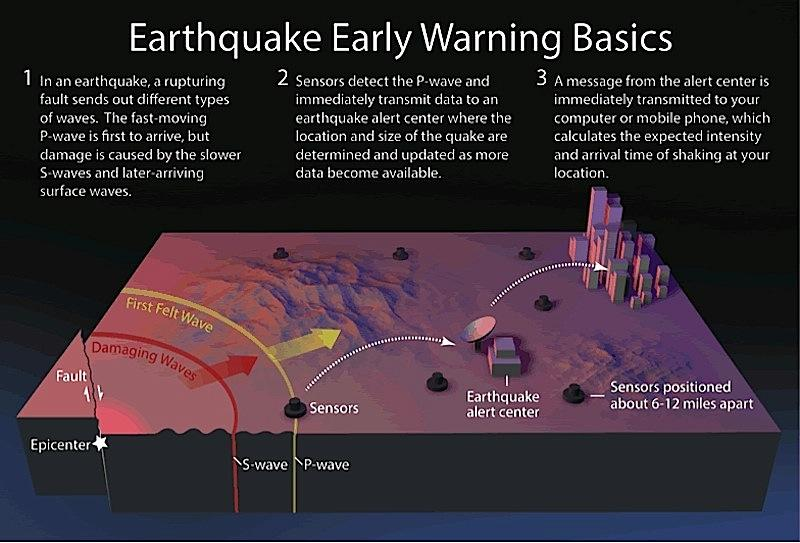
\includegraphics[scale=0.85]{98_Bilder/03_Marktsegmente/erdbeben}
%  \caption[Frühwarnsystem von Erdbeben]{Wie ein Frühwarnsystem von Erdbeben funktioniert}
%  \footnotesize Quelle: \url{http://www.ingenieur.de/var/storage/images/media/ingenieur.de/bilder/funktionsweise-fruehwarnsystems-shakealert/3666615-1-ger-DE/Funktionsweise-des-Fruehwarnsystems-ShakeAlert_image_width_884.jpg}, Stand: 05.11.2015
%\end{figure}
\subsection{Industrie}
Das Internet der Dinge kommt in der Industrie soweit zum tragen, dass man von Industrie 4.0 spricht. Dies soll die vierte industrielle Revolution zum Ausdruck bringen. Die Fertigungstechnologie soll informatisiert werden. Auch die Logistik soll ihre Automatisierung erleben. Erreicht wird dies, weil Maschinen untereinander kommunizieren können. Möglichst alle Sektoren einer Fabrik sollen vernetzt sein. Das Ziel der Industrie 4.0 ist die intelligente Fabrik.
%\begin{figure}[h]
%  \centering
%  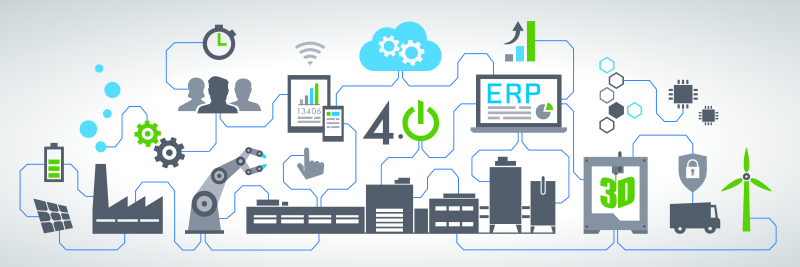
\includegraphics[scale=0.62]{98_Bilder/03_Marktsegmente/industrie4}
%  \caption[Industie 4.0 Symbolbild]{Industie 4.0}
%  \footnotesize Quelle: \url{https://www.scopevisio.com/ratgeber/wp-content/uploads/2015/11/Industrie-4.0.png}, Stand: 05.11.2015
%\end{figure}
%\newpage

\subsection{Heimautomation}
Die Heimautomation ist auch besser bekannt als Smart Home. Smart Home dient als Oberbegriff für technische Verfahren und Systeme in Wohnräumen und -häusern, in deren Mittelpunkt eine Erhöhung von Wohn- und Lebensqualität, Sicherheit und effizienter Energienutzung auf Basis vernetzter und fernsteuerbarer Geräte und Installationen sowie automatisierbarer Abläufe steht.

Unter diesen Begriff fällt sowohl die Vernetzung von Haustechnik und Haushaltsgeräten (z.B. Lampen, Jalousien, Heizung, aber auch Herd, Kühlschrank und Waschmaschine), als auch die Vernetzung von Komponenten der Unterhaltungselektronik (wie etwa die zentrale Speicherung und heimweite Nutzung von Video- und Audio-Inhalten).

Von einem Smart Home spricht man insbesondere, wenn sämtliche im Haus verwendeten Lampen, Taster und Geräte untereinander vernetzt sind, Geräte Daten speichern und eine eigene Logik abbilden können. Geräte sind teilweise auch getagged. Dies bedeutet, dass zu den Geräten im Smart Home Informationen z.B. über Hersteller, Produktnamen und Leistung hinterlegt sind. Dabei besitzt das Smart Home eine eigene Programmierschnittstelle, die (auch) via Internet angesprochen und über erweiterbare Apps gesteuert werden kann.

Eng verwandt mit diesen Verfahren und Systemen sind solche des Smart Metering, bei denen der Schwerpunkt auf dem Messen und einer intelligenten Regulierung des Energieverbrauchs liegt (vgl. \cite{wiki:smho}).
%\begin{figure}[h]
%  \centering
%  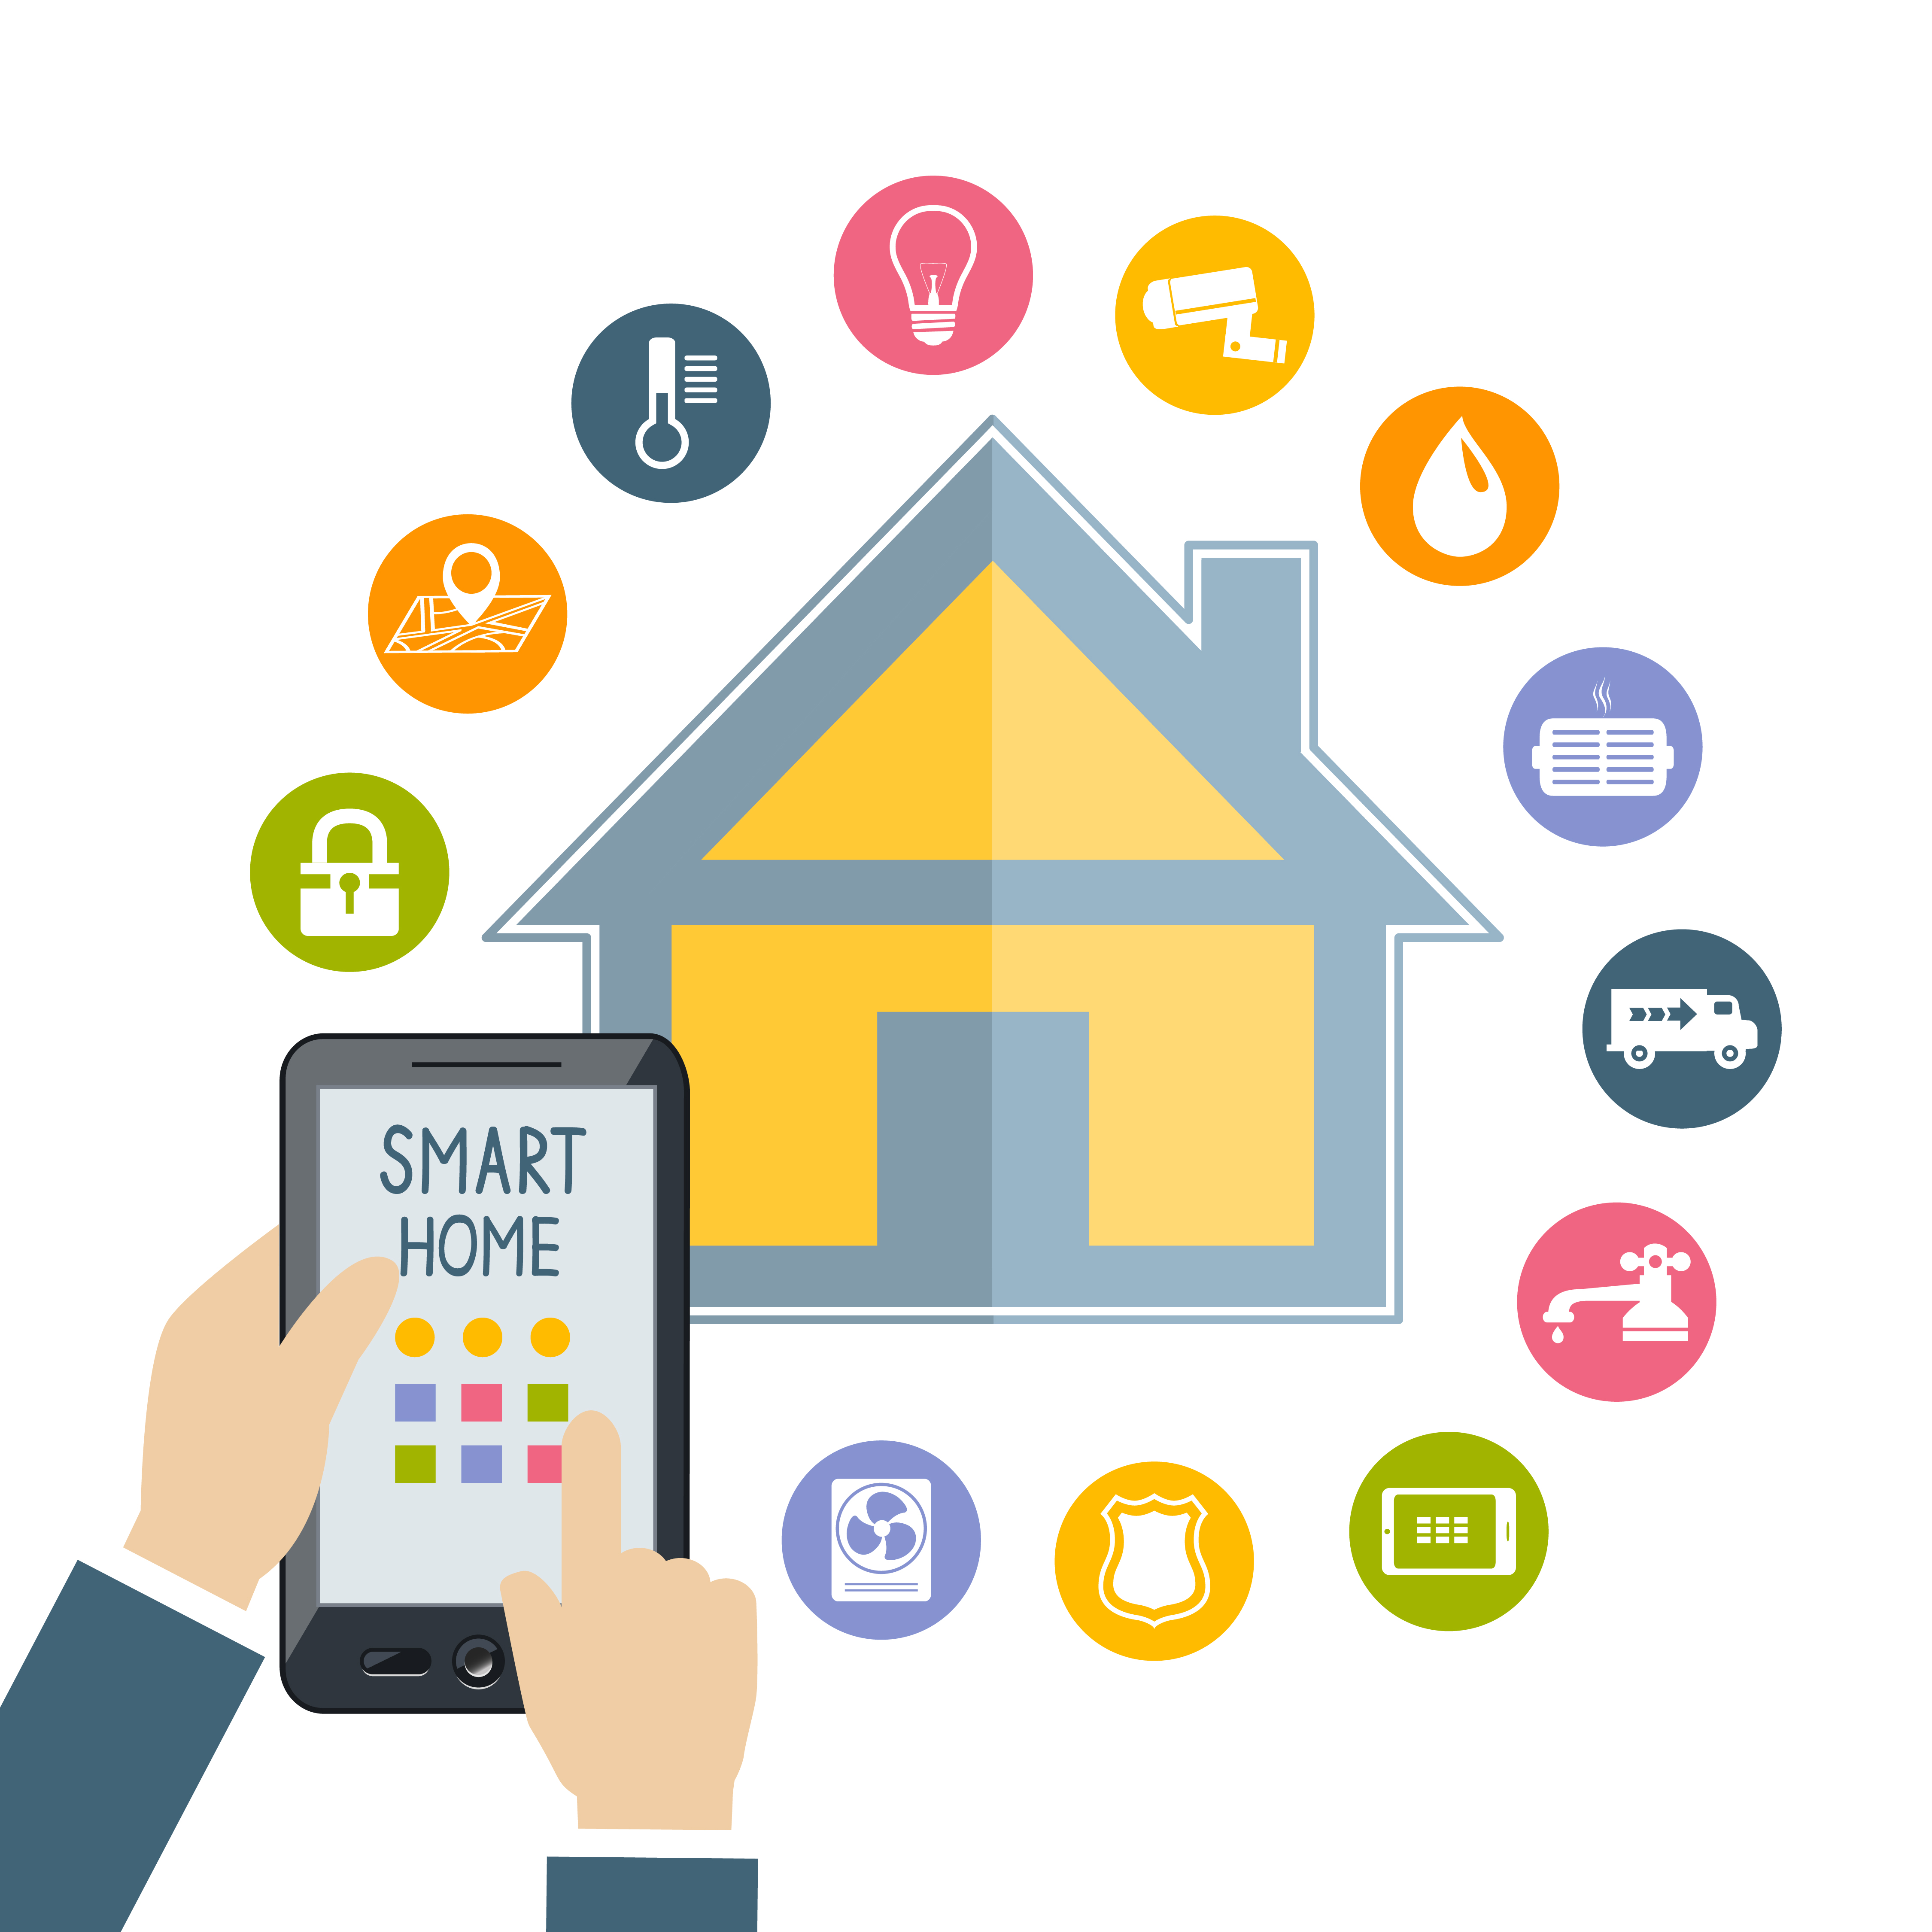
\includegraphics[scale=0.75]{98_Bilder/03_Marktsegmente/smarthome}
%  \caption[Smart Home Symbolbild]{Smart Home}
%  \footnotesize Quelle: \url{http://icon.asid.org/wp-content/uploads/2014/11/40349344_thumbnail.jpg}, Stand: 05.11.2015
%\end{figure}
%\newpage

\subsection{Automobil}
\gls{IoT} kann in vielen Bereichen der Automobilbranche eingesetzt werden. Es können wichtige Daten des Fahrzeugs ausgelesen werden, z.B. die Telemetriedaten. Diese können verwendet werden um das Fahrverhalten vom Lenker festzustellen. Des Weiteren kann, durch Nutzen der Daten, Probleme beim Auto ausgemacht und direkt Fahrer und Mechaniker alarmiert werden.
Interessant, für die Autobauer wie auch Autobesitzer, ist die Ortung der Fahrzeuge. Mit den aufgezeichneten geografischen Punkten kann analysiert werden, wie das Automobil verwendet wird und aktuelle verkehrsnahe Verkehrsberichte können genutzt werden. Die Vollendung der Vernetzung von Fahrzeugen ist das selbstfahrende Auto, welches alle nötigen Informationen empfängt, analysiert und verwendet, um das Ziel optimal zu erreichen.\\
Mercedes-Benz hat ein solches selbstfahrendes Forschungsfahrzeug entwickelt (vgl. \cite{mcbz:f015}). Die Abbildung 3.1 zeigt, wie das Fahrzeug durch die Sensoren einen Fussgänger erkennt und die Laserprojektionstechnik als Aktor verwendet, um dem Überquerenden die Fussgängerstreifen anzuzeigen.
\begin{figure}[h]
%  \centering
%  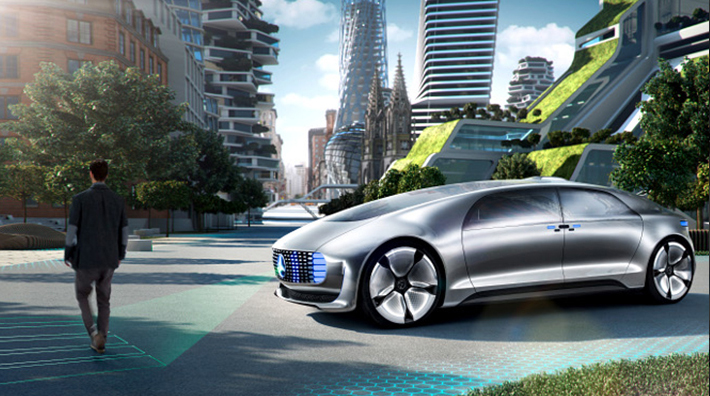
\includegraphics[scale=0.66]{98_Bilder/03_Marktsegmente/mercedesbenzf}
%  \caption[Selbstfahrendes Auto Mercedes-Benz F015 In Motion]{Das selbstfahrende Forschungsfahrzeug von Mercedes-Benz (Modell F015 In Motion)}
%  \footnotesize Quelle: \url{http://www.mercedes-benz.ch/content/media_library/f_015_luxury_in_motion_layer-gallery_1_01__710x396_01-2015.jpg}, Stand: 05.11.2015
  \centering
  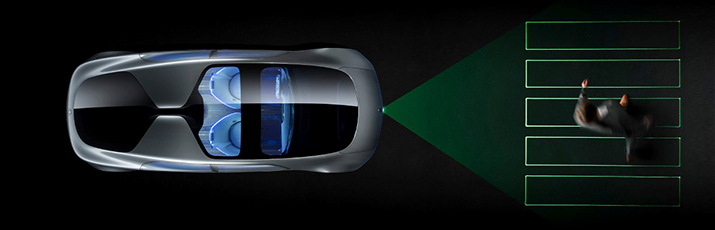
\includegraphics[scale=0.66]{98_Bilder/03_Marktsegmente/mercedesbenzf2}
  \caption[Fussgängererkennung des Mercedes-Benz F 015]{Der Mercedes-Benz F 015 erkennt Fussgänger mit seinen Sensoren}
  \footnotesize Quelle: \url{http://www.mercedes-benz.ch/content/media_library/f_015_luxury_in_motion_gallery_05_715x230_01-2015.jpg}, Stand: 05.11.2015
\end{figure}
\newpage

\subsection{Städte und Verkehr}
In Städten gibt es sehr viele Möglichkeiten. In Verbindung mit dem Verkehr geht dies ins unermessliche. Ein sehr interessantes Thema ist die Touristik. Um ein Beispiel zu nennen: Beacons, welche nötige Information an ein smartes Gerät publizieren, um Daten von der Sehenswürdigkeit abzurufen. Dazu könnte auch gleich Empfehlungen in der Umgebung notifiziert werden. So würde für die meisten Reisenden der Reiseführer wegfallen.

Ein spektakuläres Projekt ist die dynamische Strasse: \textbf{Solar Roadways}. Das sind kleine, feste Platten, welche Photovoltaik-Elementen, Elektronik, verschiedenen Sensoren und \gls{LED}s integrieren (siehe Abbildung 3.2). Die Platten können wie Pflastersteine verlegt und miteinander verbunden werden. Durch die Sonneneinstrahlung sind sie permanent und umweltschonend mit Strom versorgt. Die \gls{LED}s können zentral gesteuert werden, um so die Fahrbahnmarkierungen anzuzeigen und z.B. aus zwei breiten Spuren drei schmale machen, spontane Parkflächen oder Verkehrszeichen. Die Sensoren können feststellen, wenn Tiere oder Menschen darüber laufen und die Fahrer, schon ein paar hundert Meter vorher, über die \gls{LED}s warnen. Und die Platten sind beheizbar. Dies erhöht die Verkehrssicherheit und verringert vermutlich Baustellen. Es wurde von Privatpersonen initiiert und gecrowdfunded. Das Vorhaben ist auf Indiegogo (\url{www.indiegogo.com}) im Juni 2014 deutlich überfinanziert abgeschlossen worden. In Holland hat man im Jahr 2014 begonnen, Radwege auf diese Weise zu bauen (vgl. \cite{hoco:sorw}).
\begin{figure}[h]
  \centering
  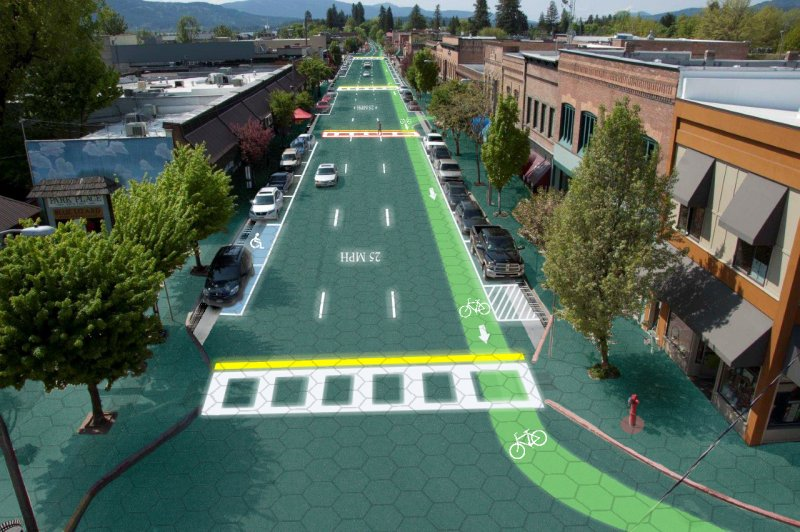
\includegraphics[scale=0.61]{98_Bilder/03_Marktsegmente/solar_roadway_00}
  \caption[Solar Roadway, dynamische Strasse]{Das Solar Roadway verändert die Strasse für die aktuelle Verkehrsituation}
  \footnotesize Quelle: \url{http://www.solarroadways.com/images/intro/Downtown%20Sandpoint%202%20-%20small.jpg}, Stand: 05.11.2015
\end{figure}
%\newpage
%\begin{figure}[H]
%  \centering
%  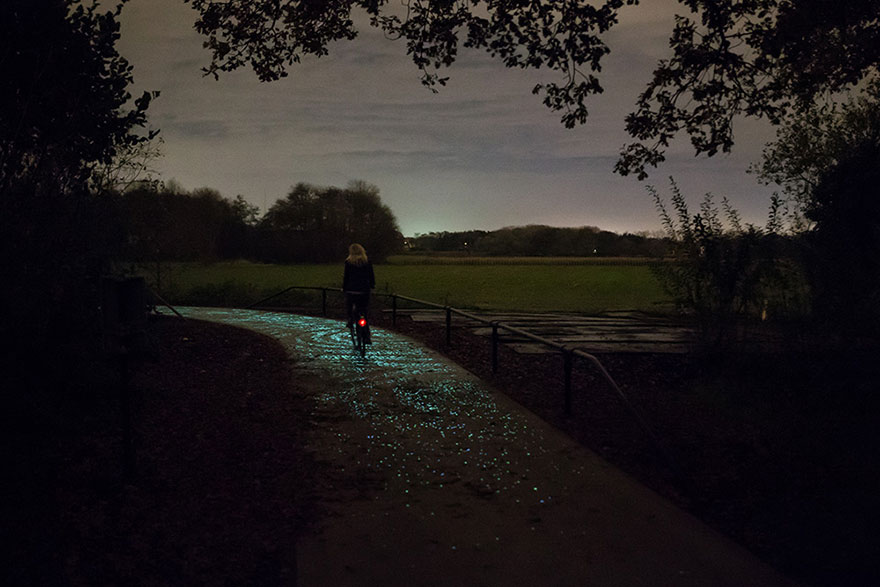
\includegraphics[scale=0.5]{98_Bilder/03_Marktsegmente/solar_roadway_02}
%  \caption[Solar Roadway in der Dämmerung]{Solar Roadway: In der Dämmerung wird der Weg an den nötigen Stellen beleuchtet}
%  \footnotesize Quelle: \url{http://static.boredpanda.com/blog/wp-content/uploads/2014/11/van-gogh-starry-night-glowing-bike-path-daan-roosengaarde-2.jpg}, Stand: 05.11.2015
%  \centering
%  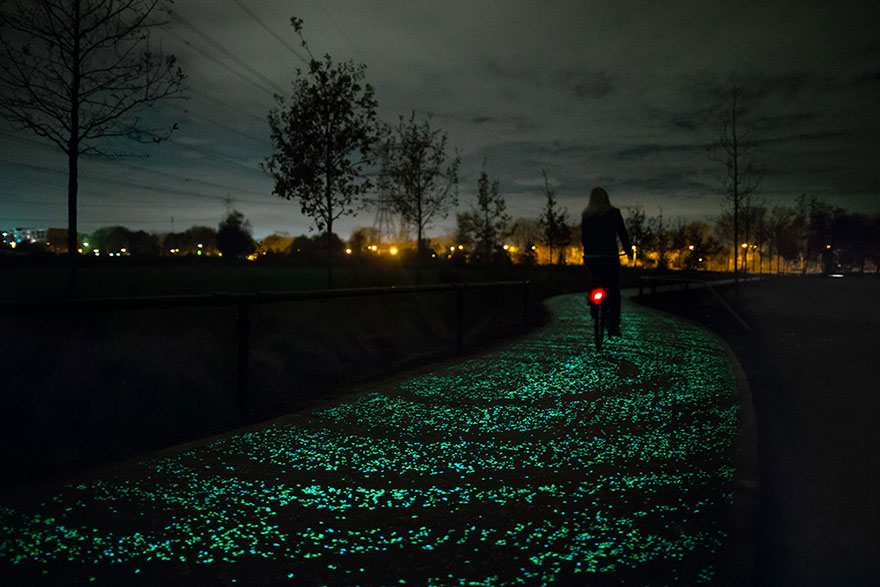
\includegraphics[scale=0.5]{98_Bilder/03_Marktsegmente/solar_roadway_01}
%  \caption[Solar Roadway bei Nacht]{Solar Roadway: Bei Nacht ist der Veloweg komplett beleuchtet}
%  \footnotesize Quelle: \url{http://static.boredpanda.com/blog/wp-content/uploads/2014/11/van-gogh-starry-night-glowing-bike-path-daan-roosengaarde-1.jpg}, Stand: 05.11.2015
%\end{figure}
\newpage

\subsection{Detailhandel}
Im Verkauf hat die Revolution schon teilweise begonnen. Die grossen Unternehmen in der Schweiz beginnen alle ihre Filialen mit \gls{WLAN} auszustatten. Momentan bieten diese den \gls{WiFi} Zugang zur freien Verfügung den Kunden an. Somit steht der Kommunikationskanal für das \gls{IoT} im Laden bereit und die Kunden sind zur gegebenen Zeit bereits verbunden damit.
Weiter werden heutzutage Selbstbezahlkassen eingesetzt. Momentan werden zwei Modelle verfolgt. Eine Einkaufsart ist: Der Kunde wählt seine Produkte und scannt diese selber ein, bezahlt mit Karte oder Bar und verlässt das Geschäft. Bei der \gls{IoT} näheren Methode, registriert sich der Konsument beim Eingang an einem Terminal und rüstet sich mit einem mobilen Strichcodeleser der Filiale aus oder nimmt sein Smartphone als Scanner. Die Person liest alle Produkte mit dem Scanner ein und bezahlt, beim verlassen des Ladens, am Bezahlterminal. Beim abmelden des Scanners wird der Kunde ermittelt und das Total eingefordert.\\
Ein weiterer Schritt ist hier, alle Produkte mit einer \gls{RFID} zu taggen. Somit könnte der Kunde nur seine Kreditkarte registrieren, die Ware in den Einkaufskorb legen und die Filiale verlassen. Beim verlassen wird durch die Information auf dem \gls{RFID} Tag gemerkt, welche Ware mitgenommen wurde und die Kreditkarte wird automatisch belastet.
%\begin{figure}[H]
%  \centering
%  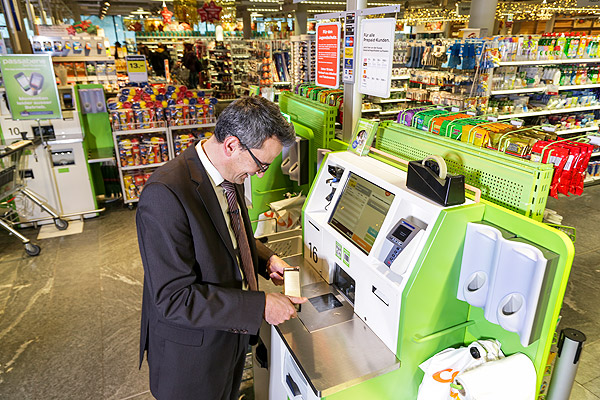
\includegraphics[scale=0.81]{98_Bilder/03_Marktsegmente/self_checkout}
%  \caption[Self Checkout Kasse]{Eine Selbstbezahlkasse für mit mobilen Scanner oder zum selber einlesen}
%  \footnotesize Quelle: \url{https://www.cooperation.ch/site/presse/get/12946772/Sutter-Selfscan_198B0923.jpg}, Stand: 05.11.2015
%\end{figure}

\section{Marktsegmente für Smartwatches}
\begin{tabbing}
xxxxxxxxxxxxxxxxxxxx\=xxxxxxxxxxxxxxxxxxxxxxxx	\kill
Mensch:		          \> Blutdruck, Puls, Bewegungen, Schlafüberwachung, Lebensüberwachung, \\\>Sportbeobachtungen, Sporttracking \\
Zeit:			          \> Individuelle Zeitansichten, Zeitfunktionen \\
Benachrichtigung:	  \> Informationen am Handgelenk, Kommunizieren
\end{tabbing}
Momentan werden Smartwatches hauptsächlich zu Notifikationszwecken und Fitnesstracking des Menschen genutzt. Noch wird das Potenzial nicht ausgenutzt Smartwatches in vielen anderen Segmenten einzusetzen. Um dies zu ermöglichen müssen die Bedürfnisse zuerst erkannt oder geschaffen werden.

\subsection{Mensch}
Heute werden Smartwatches verwendet, um den Menschen bei Aktivitäten überwachen zu können. Diese Wearables verfügen viele eingebaute Sensoren, die die Bewegungen des Trägers analysieren und dem interessierten die Daten zur Verfügung stellen. Zu den Sensoren gehören z.B. ein Bewegungssensor, Schrittzähler, Herzfrequenzmesser und viele mehr. Viele Hersteller von Smartwatches rüsten Ihre Produkte mit Sensoren und mit Auswertungsapplikationen (z.B. Google Fit, Apple Health oder Motorola Moto Body) aus. Mit diesen Apps kann der User seine Daten während dem Training auf der Uhr verfolgen oder später auf dem Smartphone auswerten. Dies macht zusätzliche Sport-/Pulsuhren überflüssig.

\subsection{Zeit}
Die Hauptaufgabe einer Uhr ist es, die Uhrzeit genau anzuzeigen. Die Smartwatches haben nicht nur die Möglichkeit die aktuelle Uhrzeit anzuzeigen, sondern auch als Weltuhr, Stoppuhr und Countdown-Rechner zu fungieren. Dabei hat der Träger der Computeruhr die Wahl, wie das Ziffernblatt aussehen soll. Wie individuell sie gestaltet werden wird vom Benutzer oder Entwickler bestimmt. Für Individualisten ist sie sehr geeignet.
%\begin{figure}[H]
%  \centering
%  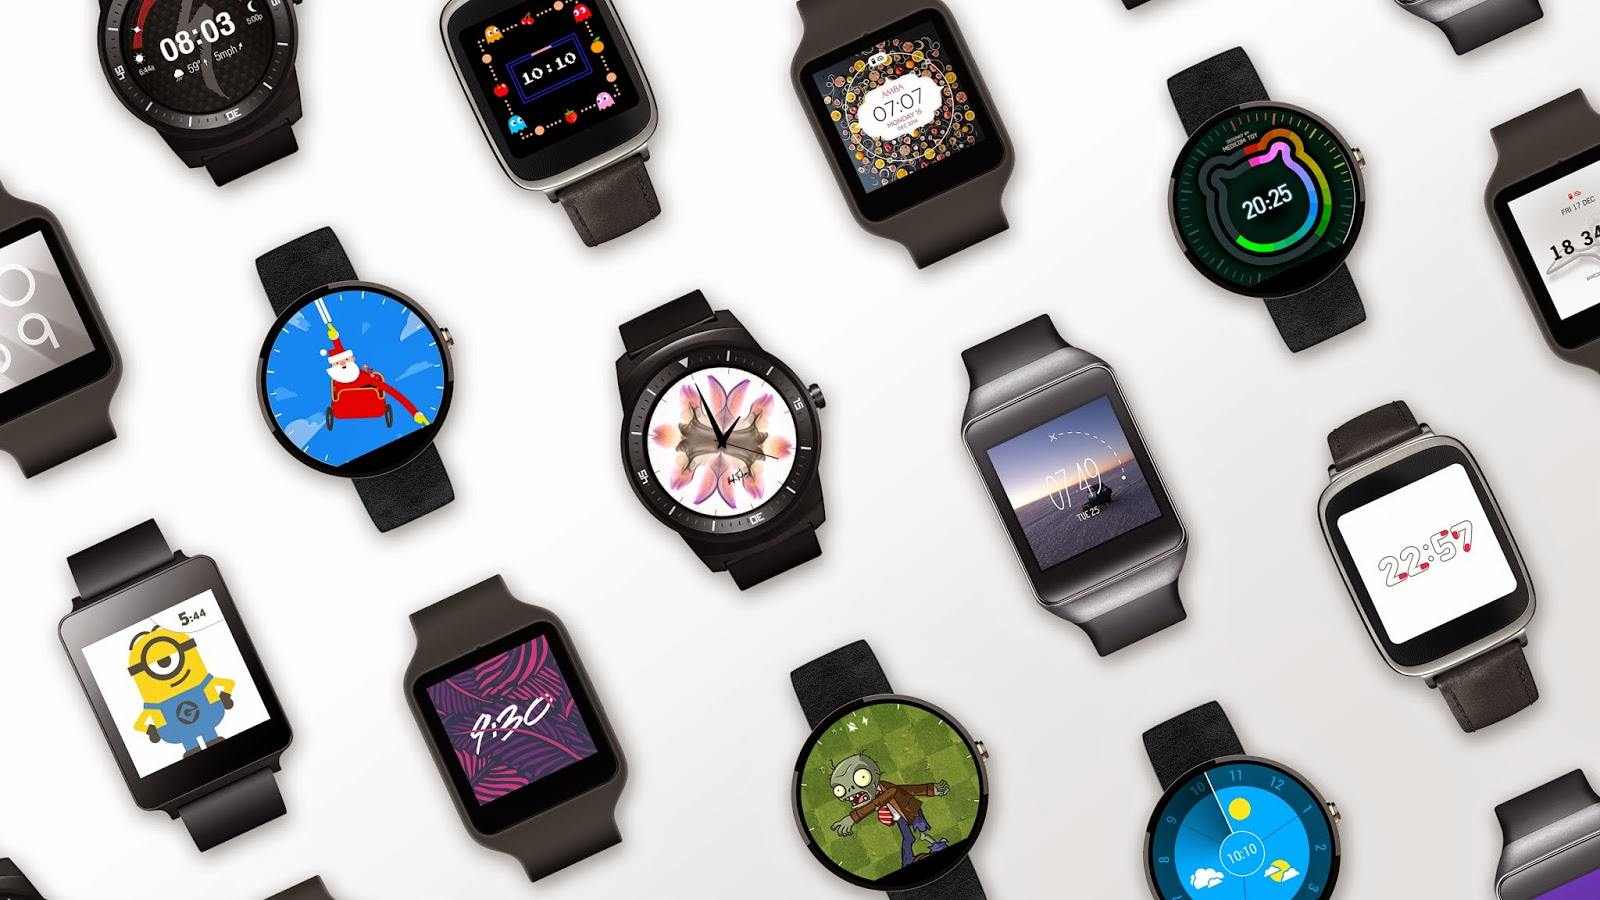
\includegraphics[scale=0.25]{98_Bilder/03_Marktsegmente/smartwatchfaces}
%  \caption[Smartwatch Ziffernblätter]{Das Ziffernblatt der meisten Smartwatches kann individuell gestaltet werden}
%  \footnotesize Quelle: \url{http://i1-news.softpedia-static.com/images/news2/Google-Launches-Watch-Face-API-You-Can-Customize-Your-Smartwatch-467130-2.jpg}, Stand: 12.11.2015
%\end{figure}

\subsection{Benachrichtigung}
Eine Smartwatch wird neben der Uhrzeitfunktion auch als Notifikationsbildschirm verwendet. Alle relevanten Benachrichtigungen an ein Smartphone können auch von der Smartwatch angezeigt werden. Dabei dient die Uhr meist als verlängerter Arm des Mobilgerätes. Es können Nachrichten empfangen, Telefonate geführt, Erinnerungen ausgelöst, der Wecker gestellt werden oder anzeigen was auf dem Smartphone ausgeführt wird, z.B aktuell abgespieltes Musikstück.
%\begin{figure}[H]
%  \centering
%  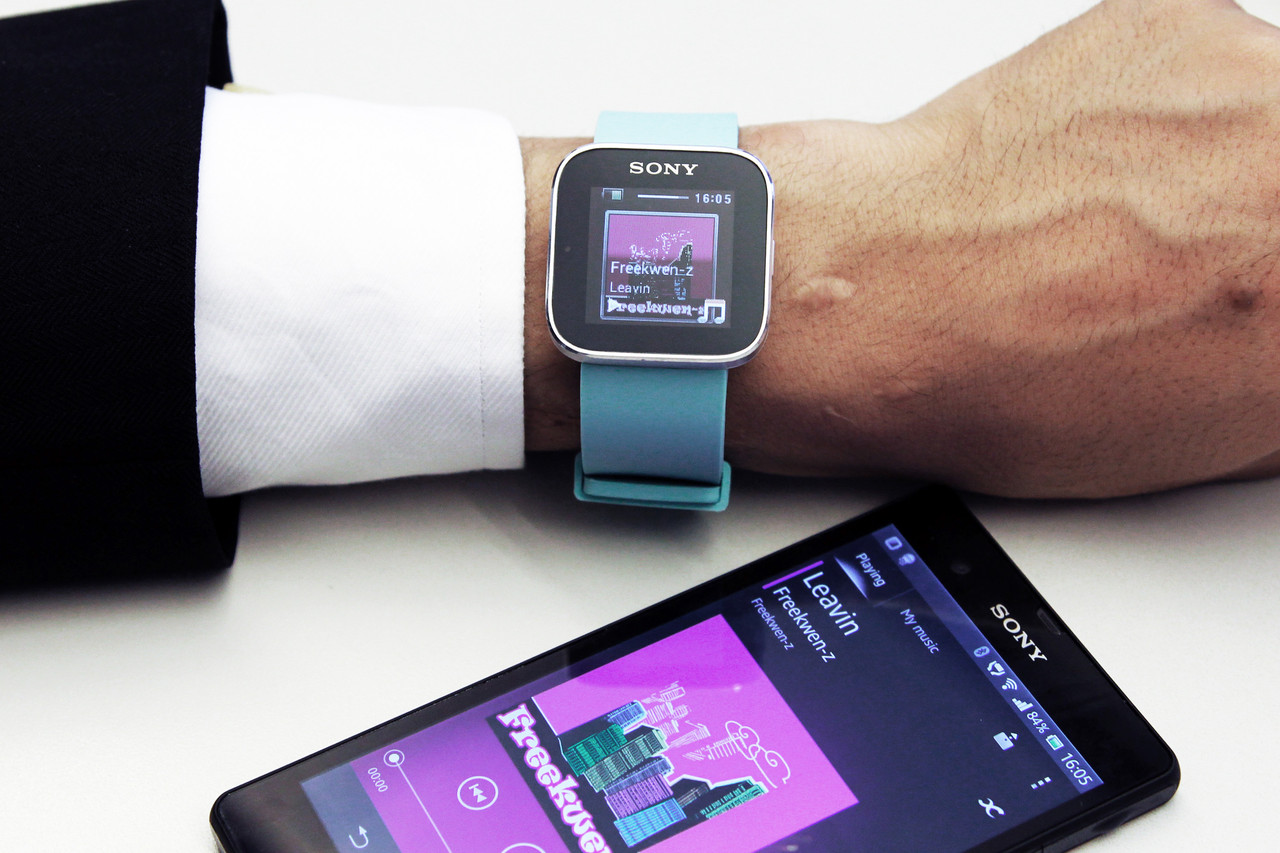
\includegraphics[scale=0.3]{98_Bilder/03_Marktsegmente/notifications}
%  \caption[Smartwatch Anzeige von Smartphone]{Die Smartwatch zeigt an, welches Musikstück auf dem Smartphone abgespielt wird}
%  \footnotesize Quelle: \url{http://smartwatchpro.it/wp-content/uploads/2015/08/OB-YT760_smartd_M_20130904020012.jpg}, Stand: 12.11.2015
%\end{figure}
%\newpage

\section{Marktsegmente für Smartwatches im Internet of Things}
\begin{tabbing}
xxxxxxxxxxxxxxxxxxxx\=xxxxxxxxxxxxxxxxxxxxxxxx	\kill
Mensch:		        \> Blutdruck, Puls, Bewegungen, Schlafüberwachung, Gesundheitsbenachrichtigung \\
Benachrichtigung:	\> Alarme, Informationen \\
Heimautomation:	  \> Fernbedienung, Statusanzeigen, Alarming \\
Detailhandel:		  \> Geldbörse, Produktebezeichnung, Einkaufsliste \\
Ortsbezogen:		  \> Navigation, Ortsspezifische Informationen, Ortung, Personen in der Nähe \\
\end{tabbing}

\subsection{Mensch}
Um die Gesundheit eines Menschen zu überwachen, eignet sich eine Smartwatch sehr gut. Sie ist immer am Handgelenk und kann bei Unregelmässigkeiten Alarm schlagen. Durch die Vernetzung werden die Daten auch an anderen Geräten zur Verfügung gestellt. Eine wichtige Benachrichtigung kann von einer anderen Smartwatch oder einem Smartphone verwendet werden. Ein sich vorstellbares Szenario: Ein Paar, beide tragen eine smarte Uhr, bei einer potenziellen Gefahr, z.B. schwacher/kein Puls, Sturz, ungewöhnliche Bewegungsabläufe, wird der Andere alarmiert.

\subsection{Benachrichtigung}
Um Informationen darzustellen, eignet sich eine Smartwatch nur beschränkt so gut, wie ein Smartphone oder andere grössere Anzeigeapparate. Sie ist jedoch prädestiniert einzelne kleine Datenmengen anzuzeigen. Die im Internet der Dinge übermittelten und verwerteten Daten, können für den Menschen, auf einem praktisch sichtbaren Display am Handgelenk, angezeigt werden. Dies gewährt einen schnellen Zugriff zu den Benachrichtigungen.
%\begin{figure}[H]
%  \centering
%  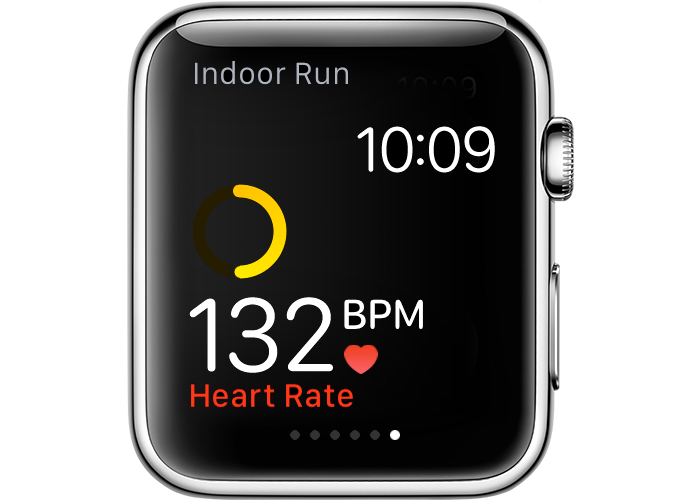
\includegraphics[scale=1]{98_Bilder/03_Marktsegmente/infodisplay}
%  \caption[Smartwatch Anzeige von Tätigkeiten]{Die Smartwatch zeigt an, welche Herzfrequenz der Träger hat und wie lange er eine Tätigkeit ausführt}
%  \footnotesize Quelle: \url{https://support.apple.com/images/en_US/applewatch/watch-indoor-workout-heartrate.png}, Stand: 20.11.2015
%\end{figure}

\subsection{Heimautomation}
Im Smart Home Bereich kann die Kombination Smartwatch und Internet of Things ihre stärken ausspielen. Durch den Zusammenschluss aller Haushaltgeräte, wie Fernseher, Lampen oder Herdplatte, sind alle Daten zentral erreichbar und verwaltbar. Nun bestehen viele Möglichkeiten die Computeruhr ins System einzubinden. Einige geeignete Anwendungsfälle sind: Das Licht ein- und auszuschalten, Alarmierung von nicht ausgeschalteten Haushaltsgeräten oder das Fernbedienen von Geräten. All dies soll unabhängig vom Ort des Uhrträgers möglich sein.

\subsection{Detailhandel}
Im Detailhandel sind besonders Finanztechnologie Applikationen schon stark vertreten, wie Apple Pay, Google Wallet oder auch die schweizerische Lösung TWINT. Diese Anwendungen erlauben Geldüberweisungen mit Smartphones oder Smartwatches mittels drahtloser Verbindung über ein Terminal, welches die Bezahlung anfordert.\\
Des weiteren könnten Smartwatches in Selbstbedienungsgeschäften als erweiterter Informationsschild von Produkten dienen. Durch die Anbindung ans Internet hat man die Möglichkeit, jedes weitere Detail, welches nicht auf der Ware beschrieben ist, auf dem Bildschirm am Arm anzuschauen. Ein sehr grosser Vorteil ist, dass verschiedene Medien genutzt werden können, z.B. detailliert Nährwertangaben, Anleitungsfilme aller Art, Explosionszeichnungen von Modellen und viele weitere.

\subsection{Ortsbezogen}
Applikationen für die Ortung oder zur Anzeige standortabhängiger Daten werden bei vielen Anwendungen benutzt. Dies auf die Smartwatch zu erweitern ist ein logischer Schritt. Ein ortsrelevantes Thema kann direkt am Handgelenk angeschaut werden ohne das Smartphone heranzuziehen.
%\begin{figure}[H]
%  \centering
%  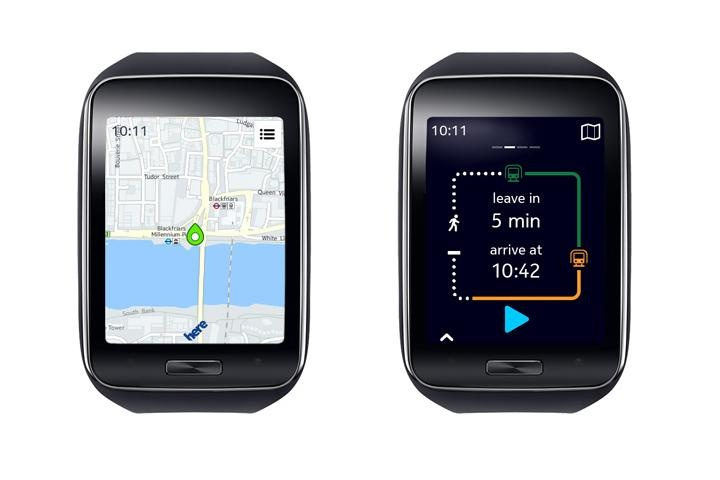
\includegraphics[scale=.5]{98_Bilder/03_Marktsegmente/watchmaps}
%  \caption[Smartwatch und ortsrelevante Informationen]{Landkarten anzeigen und ortsrelevante Informationen sind auf Smartwatches möglich}
%  \footnotesize Quelle: \url{http://icdn9.digitaltrends.com/image/here-maps-samsung-gear-s-720x480.jpg?ver=1}, Stand: 20.11.2015
%\end{figure}
